\chapter{Requirements Specification}
\label{chap:requirements_specification}

\section{Introduction}

Defining precise requirements is essential to building an enterprise-grade solution that aligns technical implementations with operational realities. This chapter details the functional and non-functional requirements, presents the global and sub-system use case models, and establishes the boundaries of the CST LePoint system.

\section{Functional Requirements}

The functional requirements cover all the actions that the system must support. To align these requirements with modern software engineering practices, they are organized into core operational modules and detailed as User Stories:

\subsection{Authentication and Authorization}
\begin{itemize}
  \item \textbf{FR-01: Secure Sign-In} (Sprint 1, 3 SP, Priority: High) \\
  As a User, I want to authenticate with credentials and SocieteId so that I can access my company scope.
  \item \textbf{FR-02: Stateless Token Generation} (Sprint 1, 2 SP, Priority: High) \\
  As a User, I want to receive a signed JWT token upon login so that my session is authenticated without server-side state.
  \item \textbf{FR-03: Token Revalidation} (Sprint 1, 1 SP, Priority: Medium) \\
  As a Client App, I want to verify the token validity on startup so that I can automatically restore active sessions.
  \item \textbf{FR-04: Granular Access Control} (Sprint 2, 5 SP, Priority: High) \\
  As an Administrator, I want to assign navigation and API permissions to roles so that users only see and execute authorized actions.
\end{itemize}

\subsection{Fleet Management}
\begin{itemize}
  \item \textbf{FR-05: Bus Registration} (Sprint 2, 2 SP, Priority: High) \\
  As an Administrator, I want to manage buses (immatriculation, model, capacity) so that they can be assigned to routes.
  \item \textbf{FR-06: Driver Assignment} (Sprint 2, 2 SP, Priority: High) \\
  As an Operator, I want to link drivers to buses and RFID badges so that operational attendance can be registered.
  \item \textbf{FR-07: Modem Association} (Sprint 2, 2 SP, Priority: Medium) \\
  As an Administrator, I want to catalog IoT modems and pair them with buses so that telemetry can be mapped to active vehicles.
\end{itemize}

\subsection{Pickup Planning}
\begin{itemize}
  \item \textbf{FR-08: Circuit Definition} (Sprint 2, 3 SP, Priority: High) \\
  As an Operator, I want to create circuits with GPS coordinates, distance, and duration so that routes can be planned.
  \item \textbf{FR-09: Ordered Pickup Points} (Sprint 2, 3 SP, Priority: High) \\
  As an Operator, I want to sequence pickup points along a circuit so that the bus follows a strict logistical route.
\end{itemize}

\subsection{Passenger and Shift Management}
\begin{itemize}
  \item \textbf{FR-10: Employee Directory} (Sprint 2, 3 SP, Priority: High) \\
  As an Administrator, I want to manage employee records, RFID tags, and geographic coordinates so that pickups can be targeted.
  \item \textbf{FR-11: Shift Configuration} (Sprint 2, 2 SP, Priority: Medium) \\
  As an Administrator, I want to define working shifts (start/end times) so that employees can be scheduled on transit routes.
  \item \textbf{FR-12: Operational Work Orders} (Sprint 2, 3 SP, Priority: Medium) \\
  As an Operator, I want to schedule site work orders for teams so that logistical transport matches factory demand.
\end{itemize}

\subsection{IoT Telemetry Ingestion}
\begin{itemize}
  \item \textbf{FR-13: Real-Time Telemetry Ingestion} (Sprint 4, 5 SP, Priority: High) \\
  As a Modem, I want to submit periodic GPS/RFID occupancy payloads to the API so that fleet status is updated in real-time.
  \item \textbf{FR-14: Telemetry Replay Protection} (Sprint 4, 2 SP, Priority: High) \\
  As a System, I want to reject telemetry payloads older than 15 minutes so that replay attacks are prevented.
  \item \textbf{FR-15: Automatic Geofence Tracking} (Sprint 4, 5 SP, Priority: High) \\
  As a System, I want to flag a bus detour if it deviates more than 250m from the route so that deviations are logged immediately.
\end{itemize}

\subsection{Real-Time Supervision}
\begin{itemize}
  \item \textbf{FR-16: Cartographic Tracking} (Sprint 3, 5 SP, Priority: High) \\
  As an Operator, I want to view active buses moving in real-time on a map so that I can supervise fleet routes visually.
  \item \textbf{FR-17: Telemetry Timeline} (Sprint 3, 3 SP, Priority: Medium) \\
  As an Operator, I want to see a chronological log of events for each bus so that I can analyze runtime alerts and updates.
\end{itemize}

\subsection{Predictive Analytics}
\begin{itemize}
  \item \textbf{FR-18: ETA Forecasting} (Sprint 4, 5 SP, Priority: High) \\
  As an Operator, I want to receive machine-learning predicted ETAs for active buses so that I can inform plants of potential delays.
  \item \textbf{FR-19: Batch ETA Calculations} (Sprint 4, 3 SP, Priority: High) \\
  As a Backend, I want to query FastAPI for ETAs of all active buses in parallel so that tracking updates remain efficient.
\end{itemize}

\subsection{Business Intelligence Reporting}
\begin{itemize}
  \item \textbf{FR-20: Dynamic Querying \& Reporting} (Sprint 5, 5 SP, Priority: High) \\
  As an Operator, I want to run historical telemetry and attendance reports with sorting, grouping, and exporting so that I can audit transport operations.
  \item \textbf{FR-21: Custom Report Layouts} (Sprint 5, 3 SP, Priority: Medium) \\
  As an Operator, I want to save my custom column groupings and configurations so that I can reload them with one click.
\end{itemize}

\section{Non-Functional Requirements}

The non-functional requirements describe the quality attributes, technological standards, and operational constraints achieved in the CST LePoint project:

\subsection{Performance and Ingestion Latency}
To handle high-frequency data generated by the active fleet, the system must adhere to strict performance targets:
\begin{itemize}
  \item \textbf{Ingestion Response Time}: Telemetry ingestion API requests (\texttt{POST /cm/bus/runtime/positions}) must be processed and resolved in under 200ms to avoid network queues on cellular IoT devices.
  \item \textbf{High Concurrency Support}: The backend must support concurrent telemetry updates from 50+ IoT modems broadcasting GPS/RFID packet data every 30 seconds without database deadlock or memory leaks.
  \item \textbf{UI Grid Load Latency}: Historical datagrids rendering thousands of telemetry trace records must complete client-side sorting, pagination, and filtering in less than 500ms using virtual scrolling and optimized EF Core query parameters.
\end{itemize}

\subsection{Scalability and Containerization Boundary}
The system architecture must support horizontal scaling as the company's fleet size grows:
\begin{itemize}
  \item \textbf{Container Separation}: Services must be isolated into independent container layers (Frontend client, .NET Core WebAPI, SQL Server 2019, and FastAPI ML prediction service) orchestrated using Docker Compose.
  \item \textbf{Stateless API Layers}: The backend application is stateless, allowing multiple instances of the .NET WebAPI container to run behind a reverse proxy (Nginx) to distribute concurrent REST traffic.
\end{itemize}

\subsection{Data Integrity and CQRS Transactional Boundaries}
Operational logs and financial reports demand absolute data consistency:
\begin{itemize}
  \item \textbf{Unit of Work Pattern}: Database mutations must be bound by transactional boundaries managed via MediatR Pipeline Behaviors. A failure in any handler step must trigger an automatic transaction rollback.
  \item \textbf{Fail-Fast Input Validation}: Before committing modifications to the persistence layer, incoming data must pass strict FluentValidation checks at the application commands boundary.
\end{itemize}

\subsection{Security, Cryptography, and Privacy Standards}
As an enterprise-grade platform, security controls are configured at both transmission and storage levels:
\begin{itemize}
  \item \textbf{Stateless Authentication}: All client-server communication must be authenticated using JSON Web Tokens (JWT) signed via HMAC-SHA256, carrying expiration times and client metadata claims.
  \item \textbf{Credential Hashing}: Passwords must never be stored in plain text. They are hashed using BCrypt, utilizing a configurable work factor to protect against brute-force attacks.
  \item \textbf{Action-Level Authorization}: System operations are restricted based on user role permissions (Read, Add, Edit, Delete) mapped dynamically to application routing modules.
\end{itemize}

\subsection{System Maintainability and DDD Architectural Styles}
To ensure long-term code quality and reduce technical debt:
\begin{itemize}
  \item \textbf{Clean Architecture Rules}: Core business logic (Domain and Application layers) must remain pure, with zero dependencies on external frameworks, SGBDs, or third-party mapping libraries.
  \item \textbf{Domain Invariants Enforcements}: Domain models must use private setters, requiring state changes to flow through explicit constructor factories and validation methods.
  \item \textbf{ULID Indexing}: Distributed, lexicographically sortable ULIDs (Universally Unique Lexicographically Sortable Identifiers) are used as primary database keys to optimize clustering indexing over classic random GUIDs.
\end{itemize}

\subsection{Robustness and Fault Tolerance}
The platform must degrade gracefully when external dependencies fail:
\begin{itemize}
  \item \textbf{ML Service Failure Handling}: If the FastAPI machine learning container becomes unreachable, the WebAPI backend must fallback to static duration heuristics based on deterministic circuit distances, logging a warning while keeping the user experience uninterrupted.
  \item \textbf{Replay Attack Defenses}: The ingestion engine must validate telemetry packet timestamps, rejecting any payload delayed by more than 15 minutes to protect against data injection.
\end{itemize}

\section{Use Case Model}

To model the interactions between users, external systems, and the CST LePoint platform, we establish a formal use case model. We identify the primary actors and external systems, present the global use case diagram, detail the sub-system use case models, and specify the operational flows of core use cases.

\subsection{Identification of Actors and External Systems}

To maintain a clean and coherent system boundary, the human interactions with the platform are structured around two primary roles, complemented by two external automated systems:

\subsubsection{Human Actors}
\begin{itemize}
  \item \textbf{Administrator}: Manages company tenant settings, user accounts, dynamic role-based access control (RBAC) permission matrices, fleet vehicle records, and hardware device registries.
  \item \textbf{Operator / Dispatcher}: Coordinates daily transit operations, including circuit and pickup stop planning, employee pickup assignments (\emph{Rattachements}), shift work orders, live cartographic tracking, arrival time forecasting, and business intelligence reporting.
\end{itemize}

\subsubsection{External Systems}
\begin{itemize}
  \item \textbf{IoT Telemetry Modem}: An onboard vehicular telematics unit (GPS/GPRS and RFID scanner) that transmits periodic position packets, timestamps, and passenger occupancy data to the backend ingestion API.
  \item \textbf{ML Prediction Engine}: A specialized FastAPI microservice that computes real-time Estimated Time of Arrival (ETA) predictions based on historical transit trajectories and current bus telemetry.
\end{itemize}

\subsection{Global Use Case Diagram}

The global use case diagram illustrates the high-level functional boundaries of the CST LePoint platform, organizing system capabilities into three logical packages: \emph{Administration \& Security}, \emph{Fleet \& Route Logistics}, and \emph{Real-Time Supervision \& BI}.

\begin{figure}[H]
  \centering
  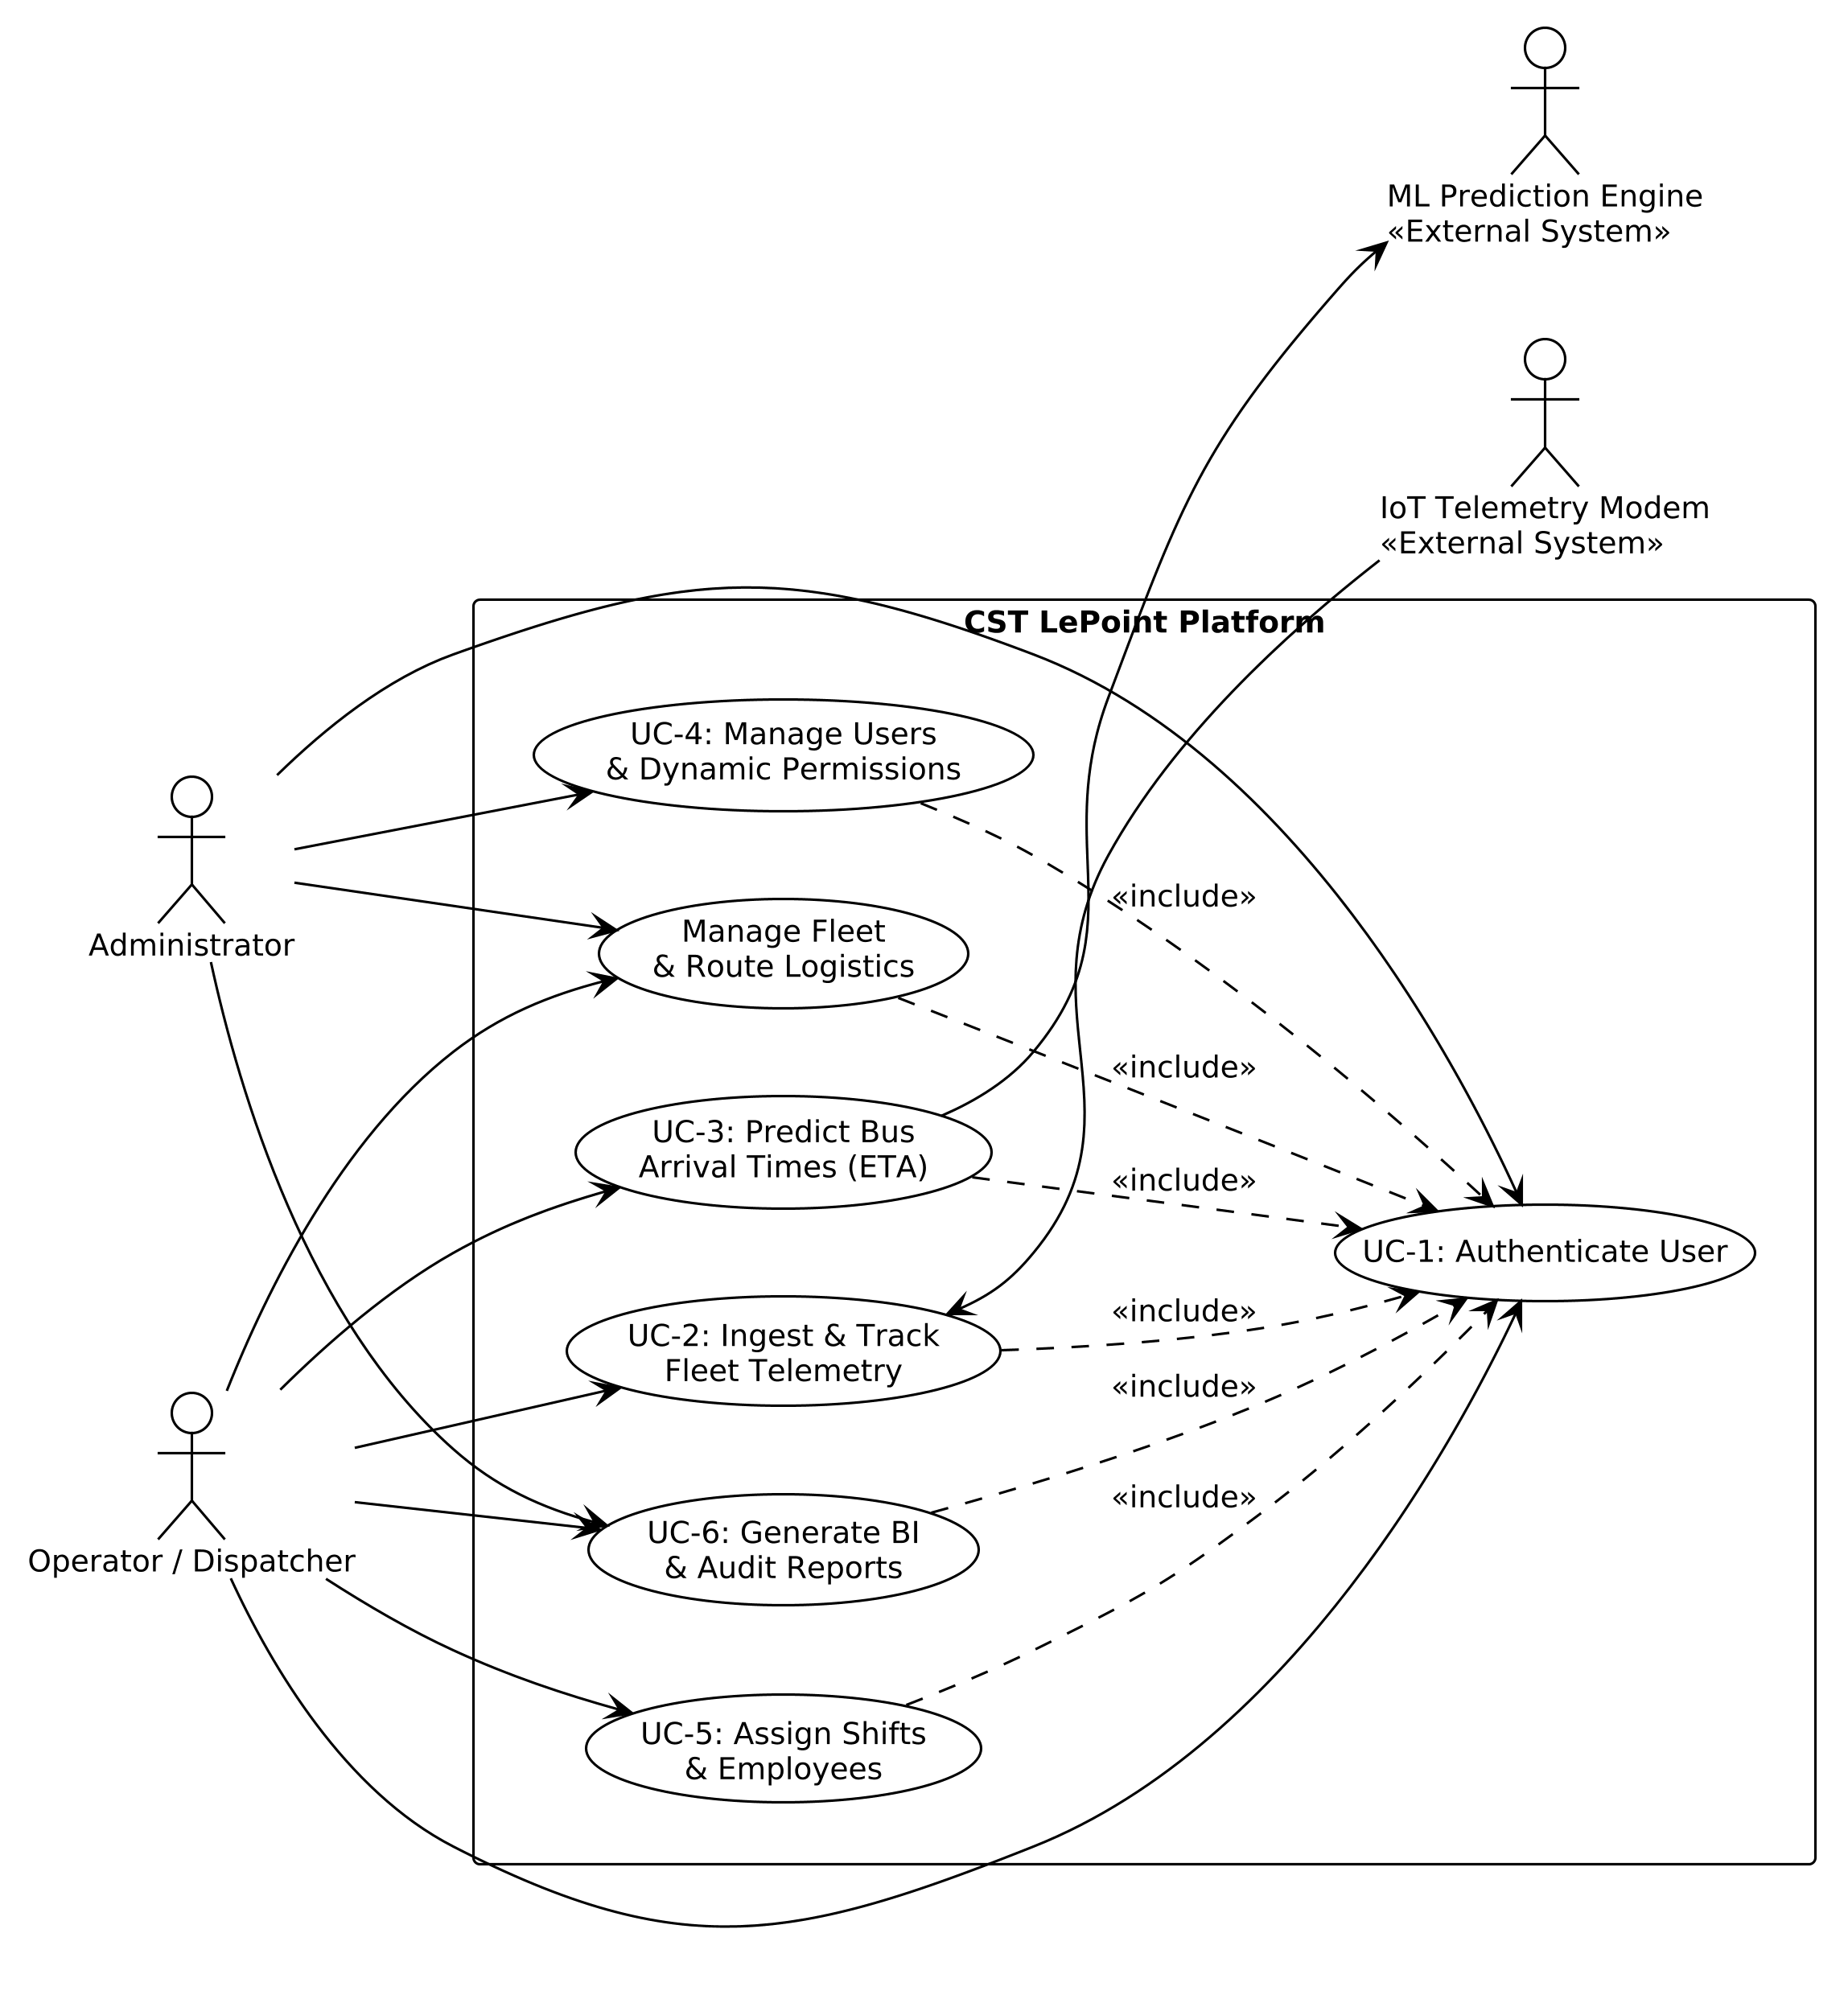
\includegraphics[width=0.85\textwidth,keepaspectratio]{figures/global-usecase.png}
  \caption{Global Use Case Diagram -- CST LePoint Platform}
  \label{fig:global-usecase}
\end{figure}

\subsection{Sub-System Use Case Models}

To provide granular visibility into specific functional areas, the system scope is decomposed into four focused sub-systems.

\subsubsection{Fleet and Route Logistics Sub-System}
This sub-system covers the management of physical vehicles, IoT modems, transit circuits, ordered pickup stations, and route allocations. Figure~\ref{fig:usecase-bus} depicts the interactions between the Administrator and Operator in configuring transport assets.

\begin{figure}[H]
  \centering
  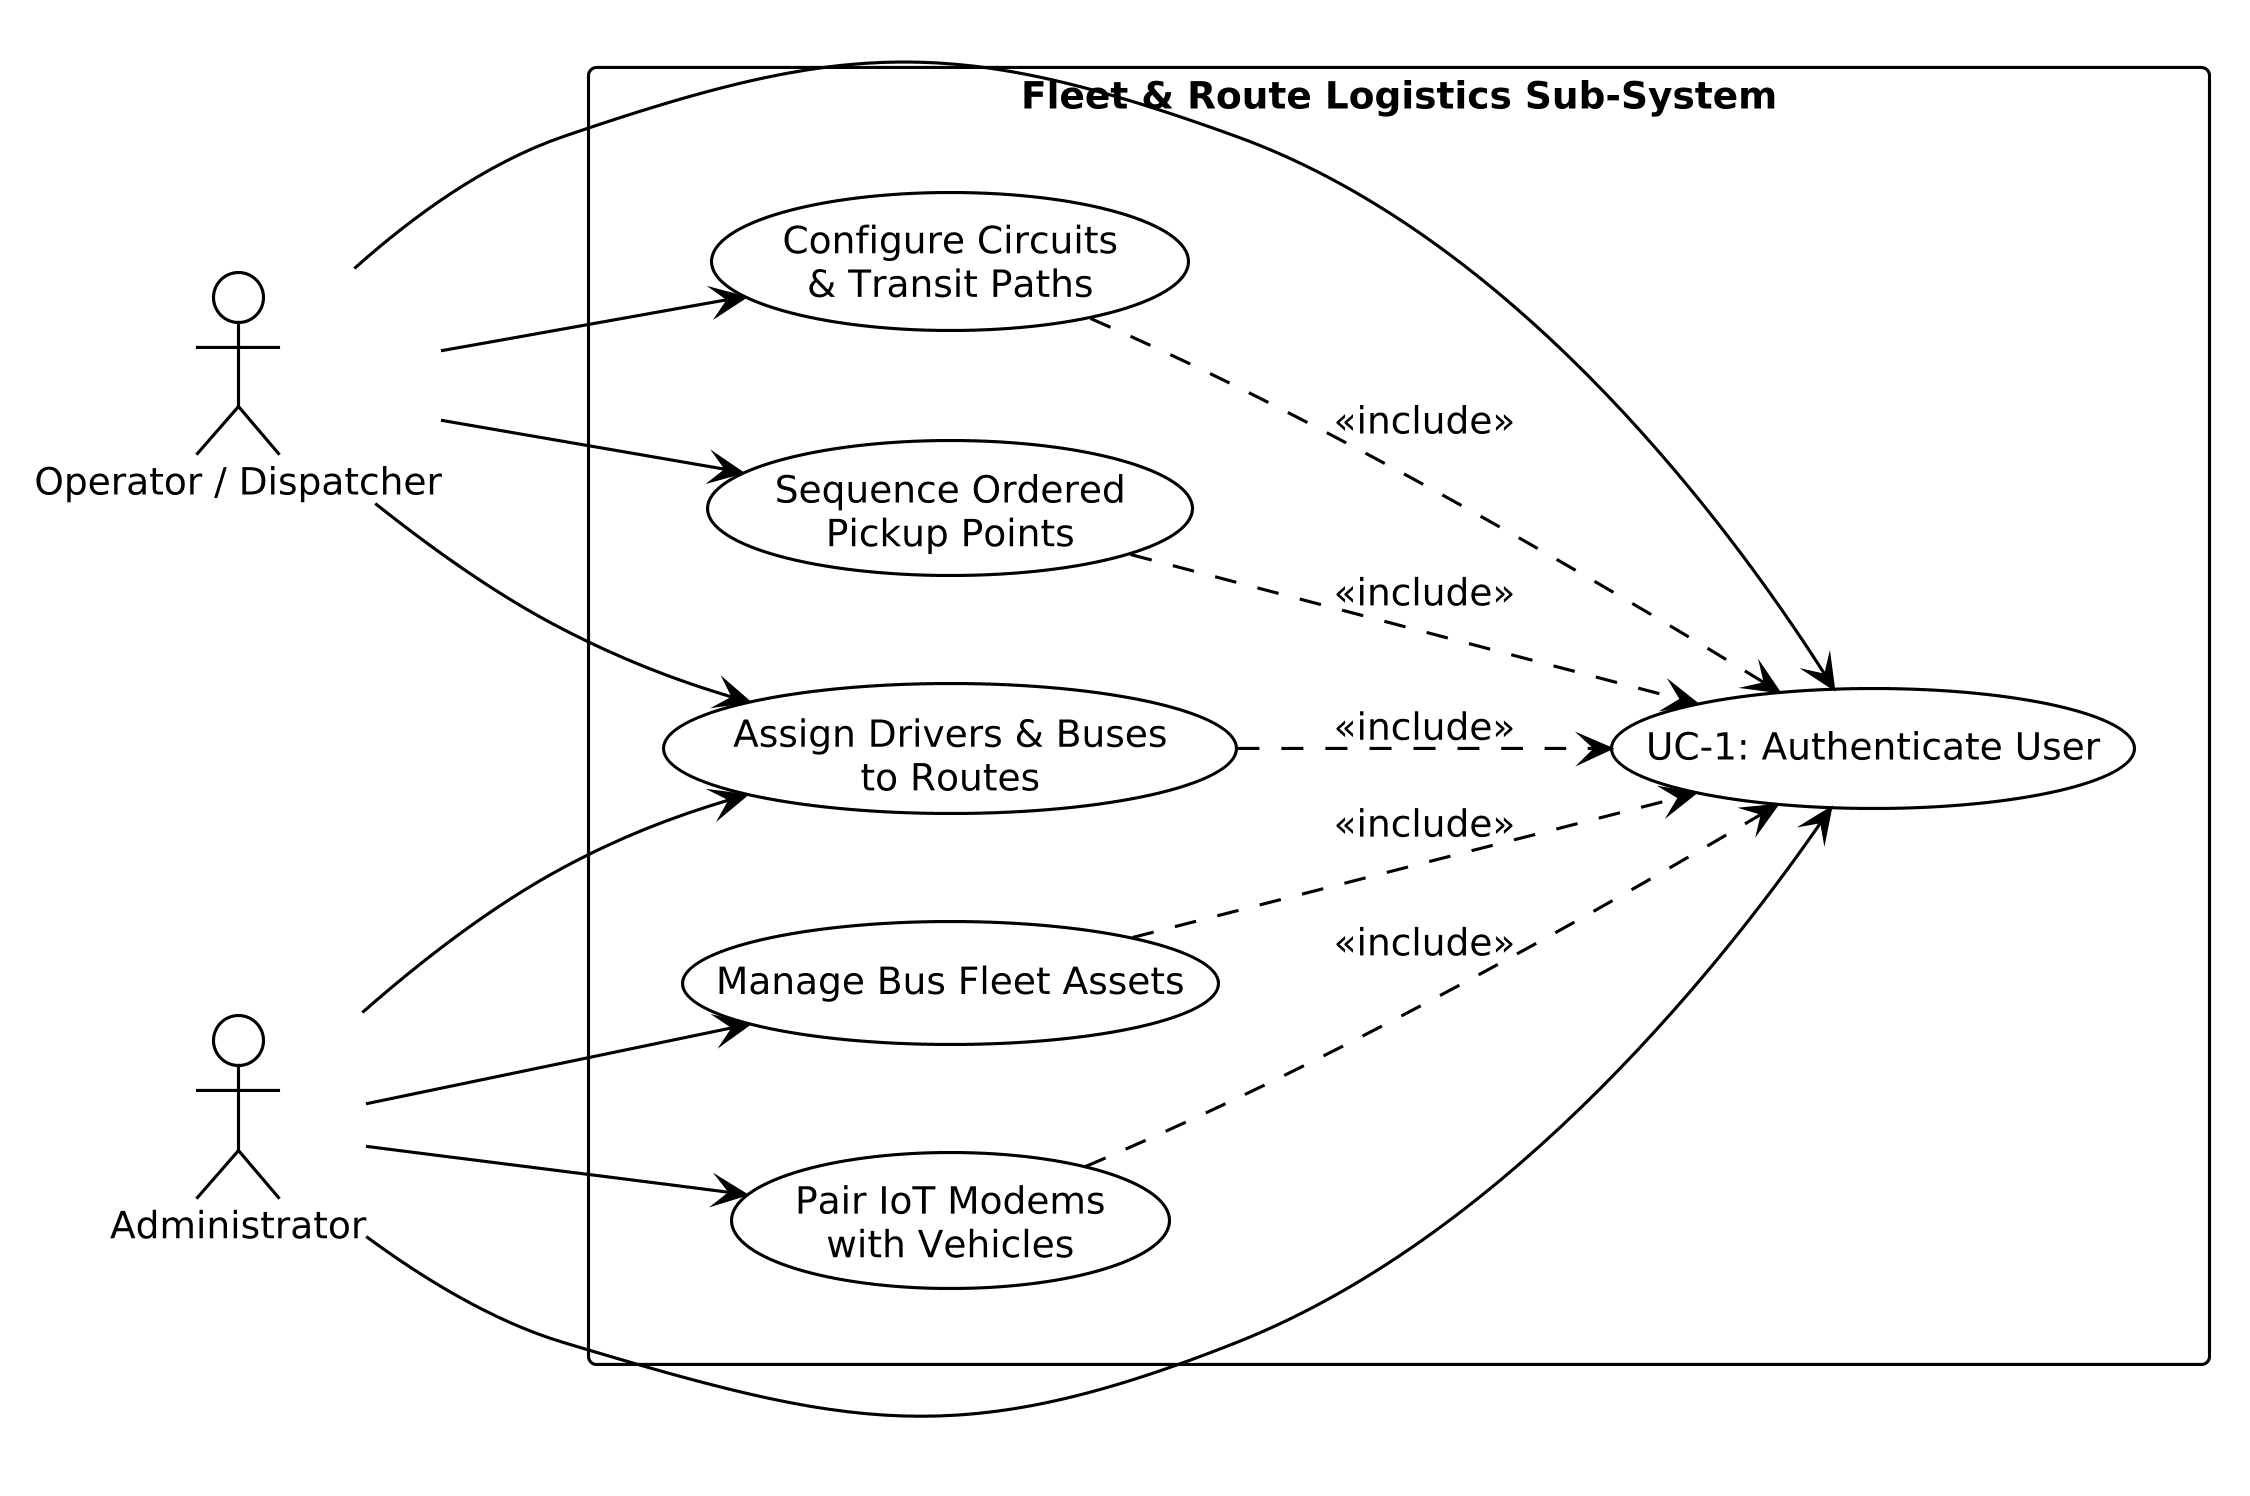
\includegraphics[width=0.80\textwidth,keepaspectratio]{figures/usecase-bus.png}
  \caption{Sub-System Use Case -- Fleet and Route Logistics}
  \label{fig:usecase-bus}
\end{figure}

\subsubsection{Real-Time Supervision and Telemetry Sub-System}
This sub-system captures high-frequency location streaming from vehicular IoT modems, evaluates geofence boundaries, renders live cartographic markers for operators, and requests ETA predictions from the machine learning engine. Figure~\ref{fig:usecase-pointcollecte} illustrates these interactions.

\begin{figure}[H]
  \centering
  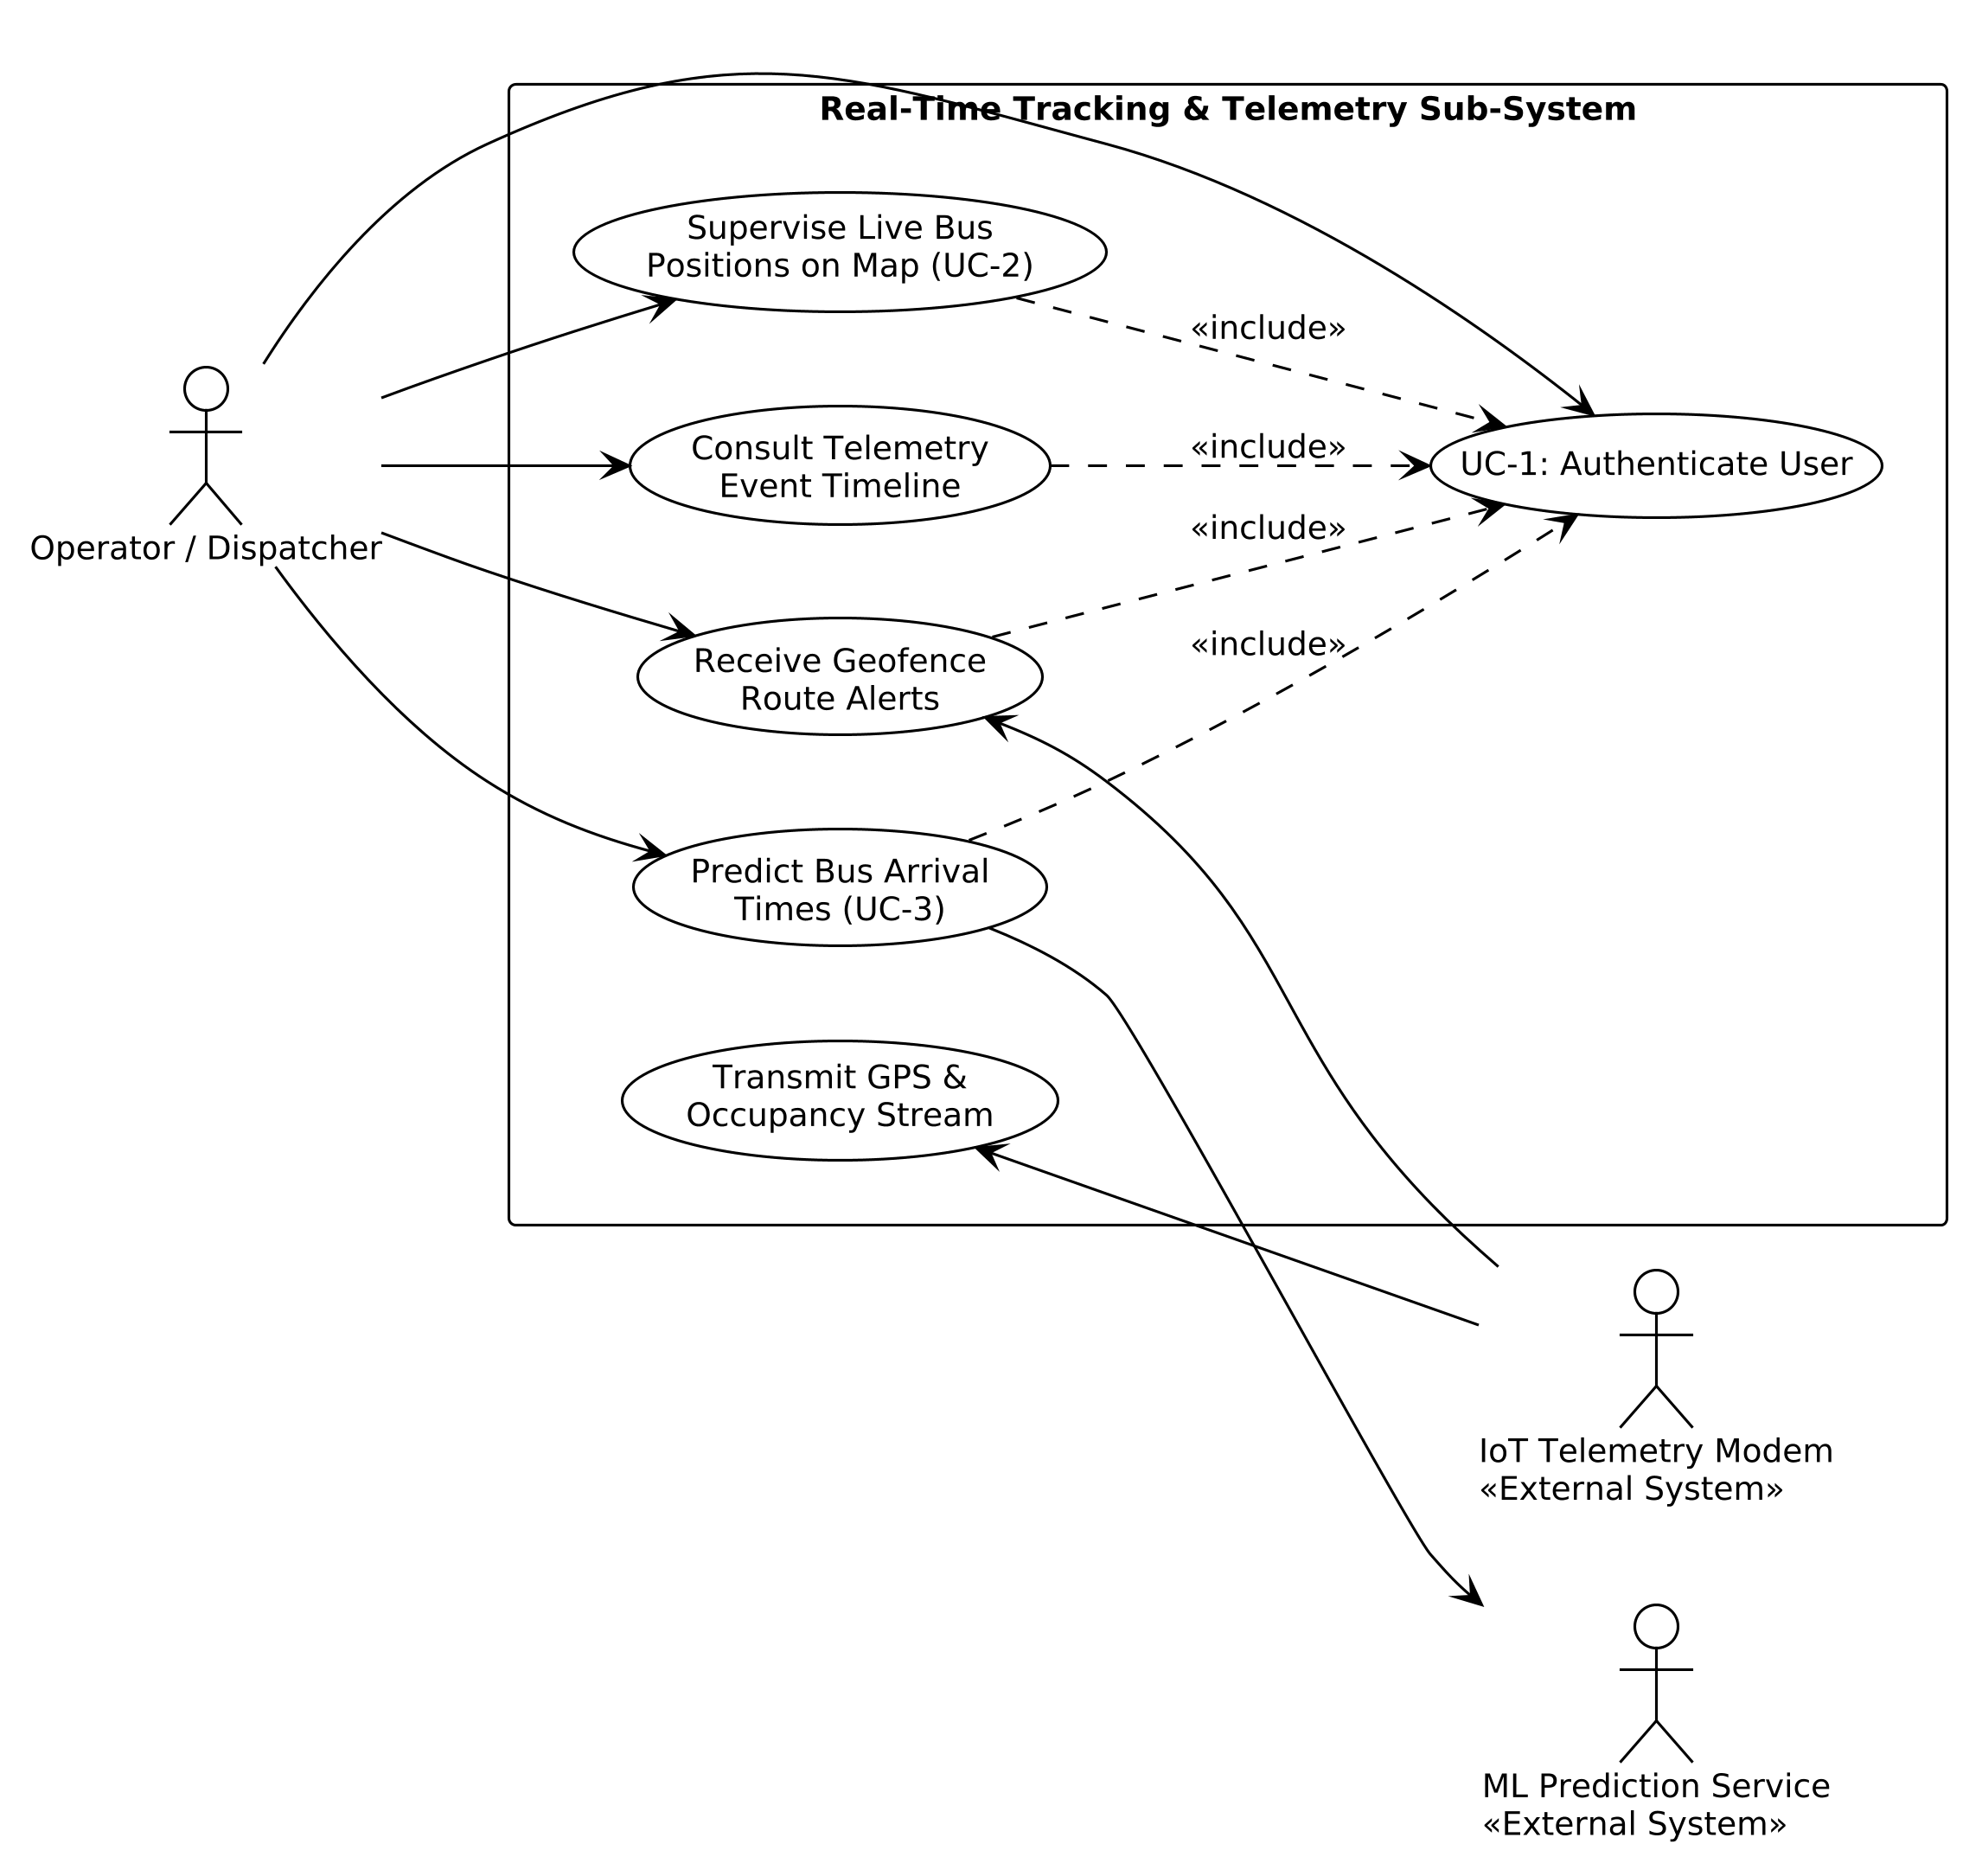
\includegraphics[width=0.85\textwidth,keepaspectratio]{figures/usecase-pointcollecte.png}
  \caption{Sub-System Use Case -- Real-Time Supervision and Telemetry}
  \label{fig:usecase-pointcollecte}
\end{figure}

\subsubsection{Operations and Workforce Logistics Sub-System}
This sub-system models employee roster assignments, work order scheduling across factory shifts, and historical business intelligence reporting with customizable layout persistence. Figure~\ref{fig:usecase-ops} presents the operational model.

\begin{figure}[H]
  \centering
  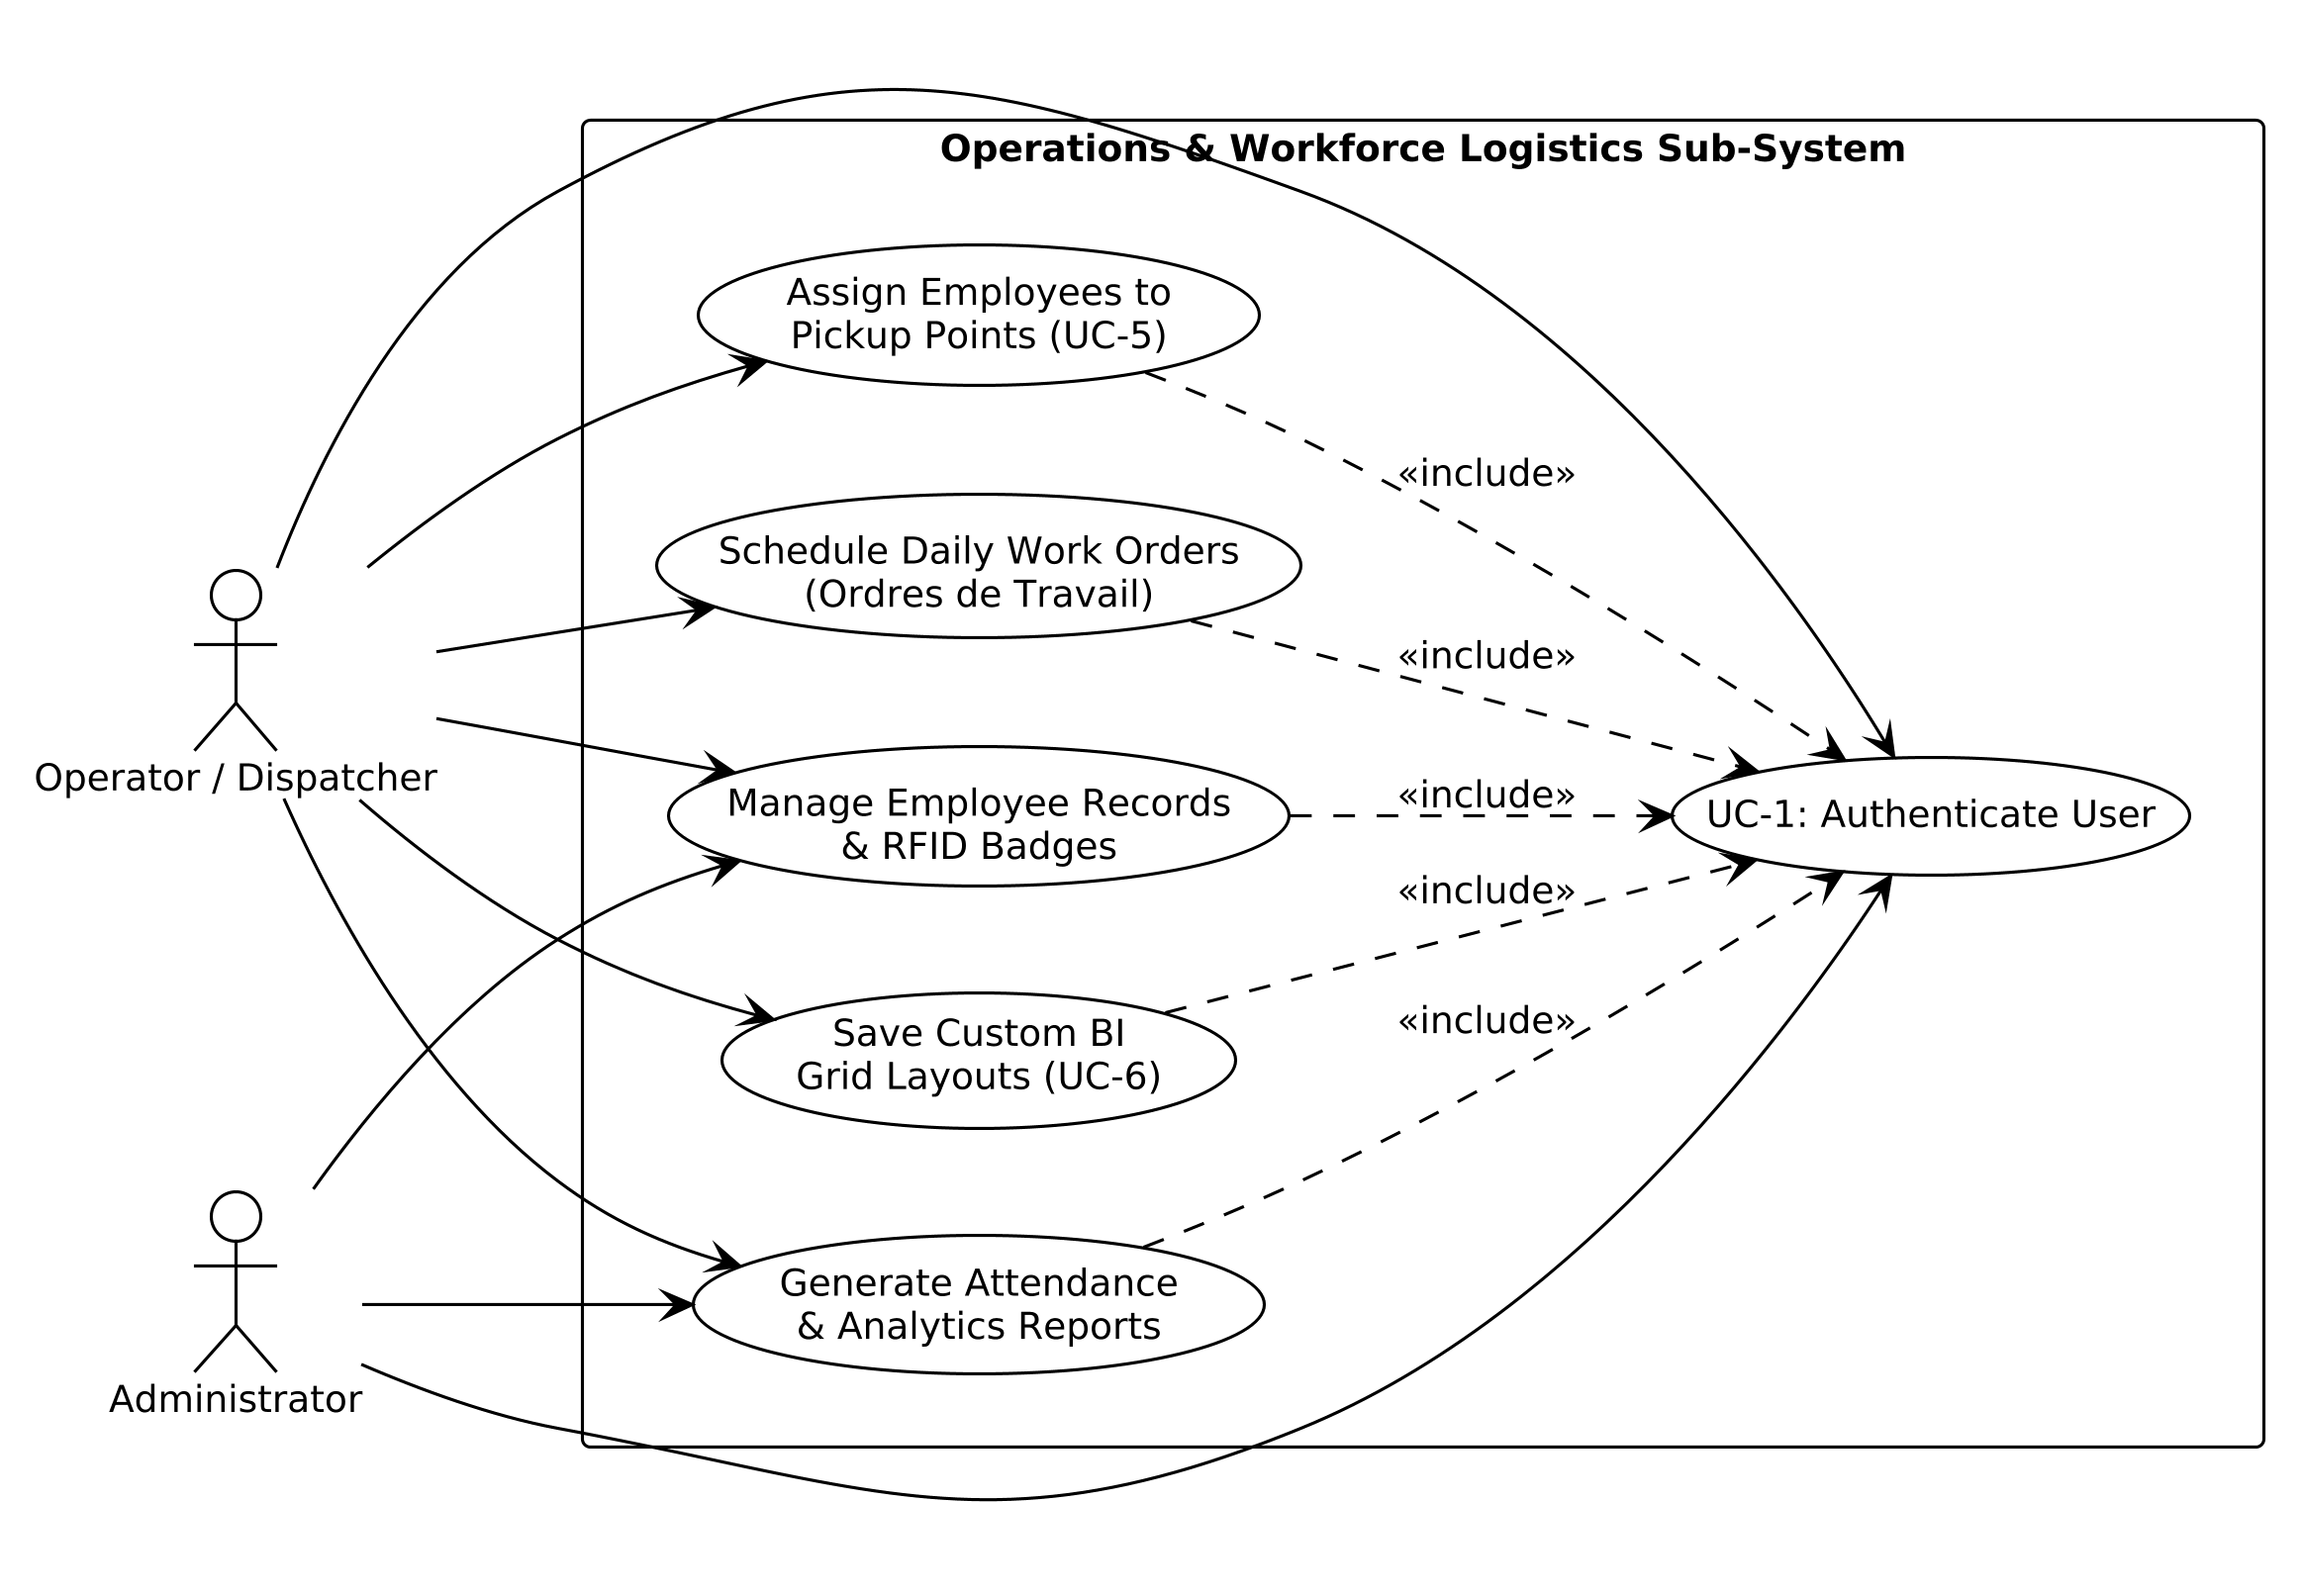
\includegraphics[width=0.80\textwidth,keepaspectratio]{figures/usecase-ops.png}
  \caption{Sub-System Use Case -- Operations and Workforce Logistics}
  \label{fig:usecase-ops}
\end{figure}

\subsubsection{System Administration and Access Governance Sub-System}
This sub-system ensures tenant isolation, user account lifecycle administration, dynamic RBAC permission matrix configuration, and reference catalog maintenance. Figure~\ref{fig:usecase-admin} illustrates the administrator workflows.

\begin{figure}[H]
  \centering
  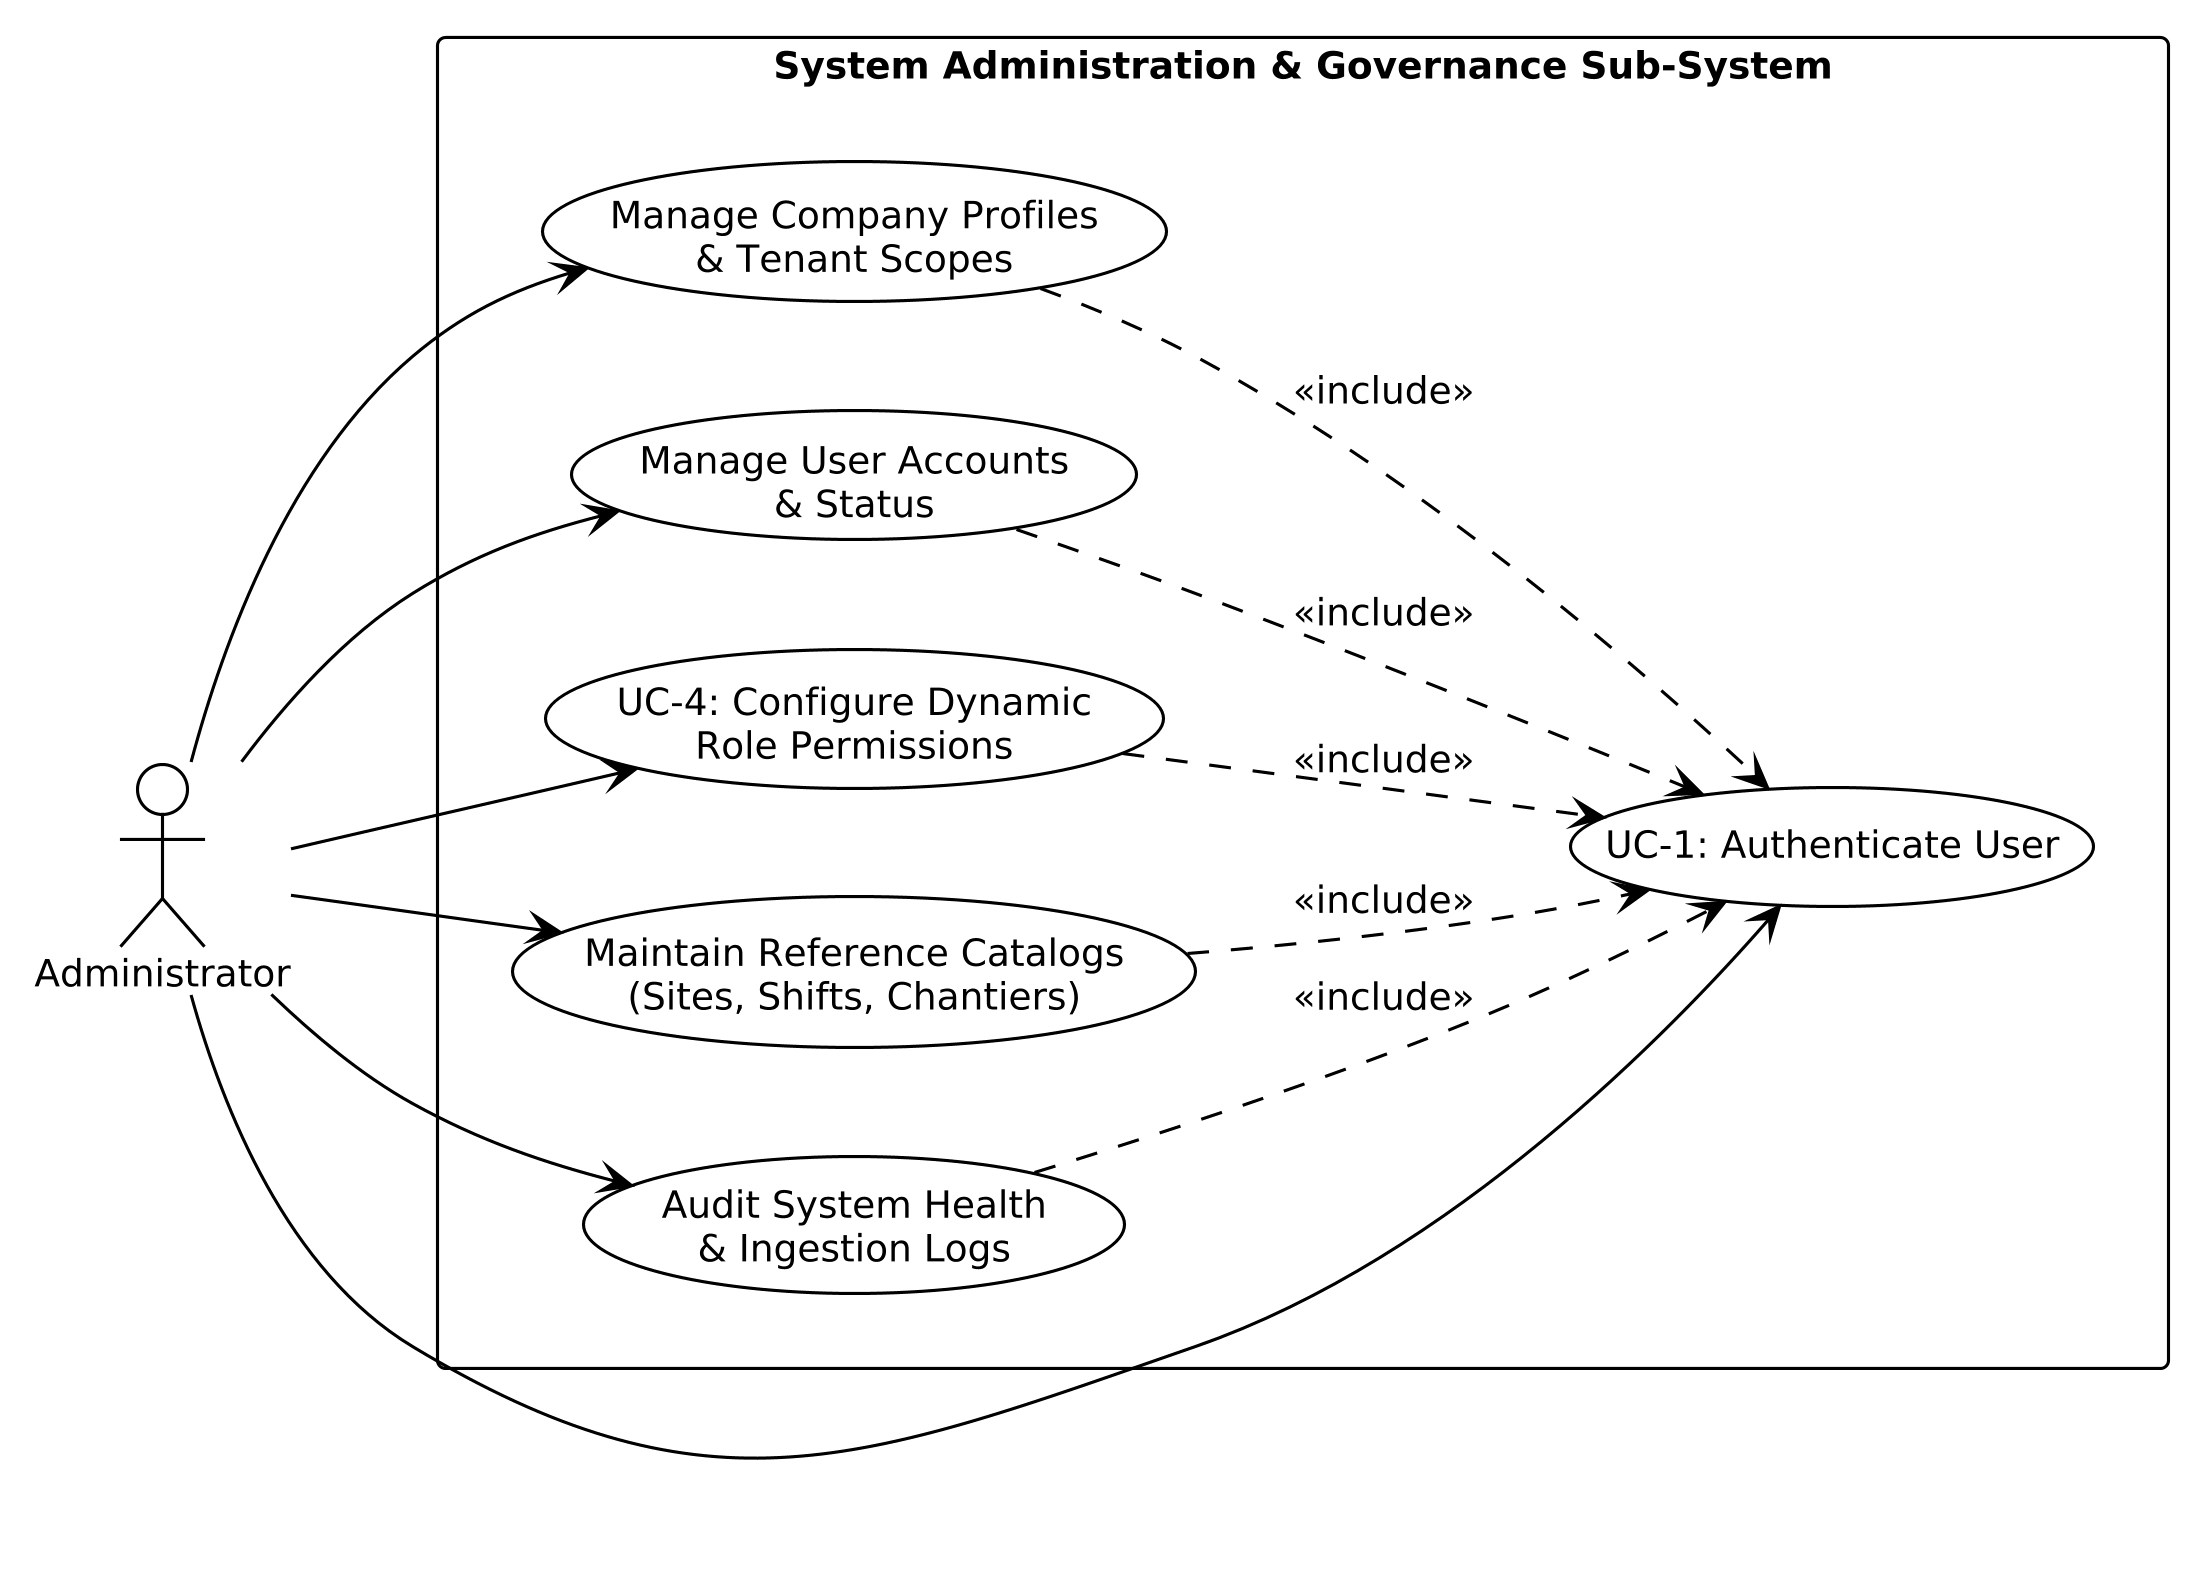
\includegraphics[width=0.75\textwidth,keepaspectratio]{figures/usecase-admin.png}
  \caption{Sub-System Use Case -- System Administration and Governance}
  \label{fig:usecase-admin}
\end{figure}

\subsection{Detailed Use Case Specifications}

This section provides formal specifications for key operational use cases developed across the platform:

\subsubsection{UC-1: Authenticate User}
\begin{itemize}
  \item \textbf{Primary Actors}: Administrator, Operator.
  \item \textbf{Preconditions}: The user account is active, and the client application is loaded at the login screen.
  \item \textbf{Postconditions}: The user session is initialized, a cryptographically signed JWT token is stored, and authorized navigation menus are displayed.
  \item \textbf{Main Flow}:
  \begin{enumerate}
    \item The user enters their username, password, and company identifier (\texttt{SocieteId}).
    \item The user submits the login form.
    \item The client application performs local validation and dispatches an HTTP POST request to \texttt{/cm/auth/login}.
    \item The WebAPI receives the payload and passes a login command to the MediatR pipeline.
    \item The command handler retrieves the user entity and verifies the password hash via BCrypt.
    \item The handler resolves the user's role and associated navigation-to-action permission matrix.
    \item The system generates an HMAC-SHA256 signed JWT Bearer token carrying identity and permission claims.
    \item The API returns an HTTP 200 OK response wrapping the token and profile metadata.
    \item The frontend stores the token and restores the user's authenticated state.
    \item The application redirects the user to the operational dashboard.
  \end{enumerate}
  \item \textbf{Alternative Flows}:
  \begin{itemize}
    \item \emph{Invalid Credentials}: If the username or password fails verification, the API returns HTTP 401 Unauthorized, and an error notification is shown.
    \item \emph{Inactive Account}: If the account is deactivated (\texttt{IsActive = false}), the API returns HTTP 403 Forbidden.
  \end{itemize}
\end{itemize}

\subsubsection{UC-2: Ingest and Track Fleet Telemetry}
\begin{itemize}
  \item \textbf{Primary Actors / Systems}: IoT Telemetry Modem, Operator.
  \item \textbf{Preconditions}: The vehicle is active, the onboard modem is initialized, and the operator has opened the live map view.
  \item \textbf{Postconditions}: Vehicle coordinates and passenger occupancy counts are committed to persistence, and live map markers are updated.
  \item \textbf{Main Flow}:
  \begin{enumerate}
    \item The onboard modem captures GPS coordinates (latitude, longitude, speed) and RFID passenger counts.
    \item The modem transmits an HTTP POST telemetry packet to \texttt{/cm/bus/runtime/positions}.
    \item The WebAPI verifies that the packet timestamp falls within a 15-minute replay-protection window.
    \item The system resolves the bus associated with the modem's 15-digit IMEI.
    \item The command handler calculates the spatial distance between the vehicle position and scheduled circuit points.
    \item The handler updates the bus runtime state and persists the telemetry record.
    \item The backend broadcasts the coordinate update via WebSocket to connected clients.
    \item The Leaflet map component updates the vehicle marker position smoothly.
  \end{enumerate}
  \item \textbf{Alternative Flows}:
  \begin{itemize}
    \item \emph{Geofence Route Deviation}: If the bus deviates more than 250 meters from the scheduled circuit path, the system logs a detour alert and generates an event record before committing.
    \item \emph{Unrecognized Modem}: If the IMEI is unregistered, the request is rejected with HTTP 404 Not Found.
  \end{itemize}
\end{itemize}

\subsubsection{UC-3: Predict Bus Arrival Time (ETA)}
\begin{itemize}
  \item \textbf{Primary Actors / Systems}: Operator / Dispatcher, ML Prediction Engine.
  \item \textbf{Preconditions}: The operator is logged in, and an active bus is in transit along a scheduled circuit.
  \item \textbf{Postconditions}: The machine learning estimated arrival time (in minutes) and confidence metrics are displayed on the tracking panel.
  \item \textbf{Main Flow}:
  \begin{enumerate}
    \item The operator clicks on an active bus marker on the live tracking map.
    \item The client issues an ETA prediction query to the backend API.
    \item The backend aggregates real-time bus telemetry (speed, current coordinates, passenger occupancy, capacity, and circuit ID).
    \item The backend issues an HTTP POST prediction request to the FastAPI microservice (\texttt{http://ml-service:8001/predict/eta}).
    \item The FastAPI microservice loads the trained regression model artifacts, executes inference, and returns the predicted ETA duration in minutes.
    \item The backend WebAPI receives the prediction response and formats it into the API contract.
    \item The tracking panel displays the remaining arrival time and estimated arrival timestamp.
  \end{enumerate}
  \item \textbf{Alternative Flows}:
  \begin{itemize}
    \item \emph{ML Service Unavailable}: If the FastAPI container is unreachable, the backend logs a warning and falls back to a deterministic distance-to-speed heuristic calculation, ensuring uninterrupted user experience.
  \end{itemize}
\end{itemize}

\subsubsection{UC-4: Configure Role Permissions Matrix}
\begin{itemize}
  \item \textbf{Primary Actors}: Administrator.
  \item \textbf{Preconditions}: The Administrator is authenticated and navigates to the Roles and Permissions governance view.
  \item \textbf{Postconditions}: Role permissions are saved in the database as a structured JSON permission matrix.
  \item \textbf{Main Flow}:
  \begin{enumerate}
    \item The Administrator opens the role management interface.
    \item The system displays the list of roles and the module permission matrix.
    \item The Administrator selects a role to edit or creates a new role.
    \item The Administrator configures module privileges (\emph{Read}, \emph{Add}, \emph{Edit}, \emph{Delete}) across functional routes (e.g. \texttt{fichier.circuit}, \texttt{monitoring.bus-tracking}, \texttt{analyse.bi-bus}).
    \item The Administrator clicks "Save Role".
    \item The client compiles the selections into a JSON array and dispatches an HTTP POST/PATCH request.
    \item The backend handler validates uniqueness within the company tenant and persists the \texttt{RoleUtilisateur} entity.
    \item The UI displays a confirmation notification.
  \end{enumerate}
  \item \textbf{Alternative Flows}:
  \begin{itemize}
    \item \emph{Duplicate Role}: If the role name already exists within the same tenant, the API aborts with a validation error.
  \end{itemize}
\end{itemize}

\subsubsection{UC-5: Assign Employee to Pickup Point and Route}
\begin{itemize}
  \item \textbf{Primary Actors}: Operator / Dispatcher.
  \item \textbf{Preconditions}: The employee record exists with registered geographic coordinates, and the transit circuit is configured.
  \item \textbf{Postconditions}: An assignment link (\texttt{Rattachement}) is created, binding the employee to a designated pickup point and scheduled shift.
  \item \textbf{Main Flow}:
  \begin{enumerate}
    \item The operator opens the employee pickup assignment module.
    \item The system renders the pickup points map alongside unassigned employee profiles.
    \item The operator selects an employee and identifies the nearest pickup station along an active circuit.
    \item The operator assigns the employee to the chosen pickup point and associated shift.
    \item The client sends an HTTP POST request to create the \texttt{RattachementEmploye} entity.
    \item The backend verifies vehicle capacity constraints and commits the assignment record.
    \item The map highlights the updated passenger count for that pickup station.
  \end{enumerate}
  \item \textbf{Alternative Flows}:
  \begin{itemize}
    \item \emph{Overcapacity Warning}: If adding the employee exceeds the bus seating capacity, the system displays a capacity warning prompt before confirmation.
  \end{itemize}
\end{itemize}

\subsubsection{UC-6: Save Custom BI Report Layout}
\begin{itemize}
  \item \textbf{Primary Actors}: Operator / Dispatcher, Administrator.
  \item \textbf{Preconditions}: The user is authenticated and has customized a BI data grid (reordered columns, applied filters, or established groupings).
  \item \textbf{Postconditions}: The customized grid configuration JSON is persisted in the database and linked to the tenant context.
  \item \textbf{Main Flow}:
  \begin{enumerate}
    \item The user opens a business intelligence dashboard (e.g. BI Bus or BI Attendance).
    \item The user customizes grid columns, sorting criteria, and multi-level groupings.
    \item The user clicks "Save Layout".
    \item A dialog prompts for a descriptive layout title (e.g. "Monthly Overtime Audit").
    \item The user enters the name and submits the dialog.
    \item The client serializes the grid state to JSON and sends an HTTP POST request to \texttt{/cm/analyse/layouts}.
    \item The backend handler upserts the \texttt{ReportLayout} aggregate, scoped by \texttt{SocieteId}.
    \item The saved layout appears in the user's layout dropdown menu for instant recall.
  \end{enumerate}
  \item \textbf{Alternative Flows}:
  \begin{itemize}
    \item \emph{Blank Layout Name}: If the user leaves the title blank, the client displays an inline validation error.
  \end{itemize}
\end{itemize}

\section{Input Validation Constraints}

To maintain data integrity and prevent corrupt persistence writes, the CST LePoint platform enforces strict validation rules at the application boundary using FluentValidation. Inbound requests are checked against the following constraints:

\begin{itemize}
  \item \textbf{Bus Entity Constraints}:
  \begin{itemize}
    \item \texttt{NumeroIMM} (Immatriculation plate format): Required, must not exceed 50 characters, and must follow standard Tunisian plate expressions (regex: \verb|^[0-9]+-TN-[0-9]+$|).
    \item \texttt{IMEI} (Onboard modem identifier): Required, must be exactly 15 numeric digits.
    \item \texttt{Capacite} (Vehicle seating capacity): Required, must be an integer between 1 and 150.
  \end{itemize}

  \item \textbf{Employee Entity Constraints}:
  \begin{itemize}
    \item \texttt{Matricule} (HR employee identification): Required, unique, and cannot exceed 20 characters.
    \item \texttt{RFID} (Badge hardware identifier): Required, must be a valid alphanumeric hexadecimal token up to 50 characters.
    \item \texttt{Latitude/Longitude} (Home geolocation): Must fall within the geographic bounds of Tunisia (Latitude: $[30.0, 38.0]$, Longitude: $[7.0, 12.0]$).
  \end{itemize}

  \item \textbf{Circuit Entity Constraints}:
  \begin{itemize}
    \item \texttt{CodeCircuit} (Route catalog identifier): Required, unique, alphanumeric code up to 20 characters.
    \item \texttt{DistanceKm} (Transit path length): Required, must be a positive decimal value greater than 0.0.
    \item \texttt{DureeMinutes} (Estimated transit duration): Required, must be a positive integer greater than 0.
  \end{itemize}
\end{itemize}

\section{Requirements Traceability Summary}

To ensure complete coverage of the design scope, we cross-reference our functional requirements with the corresponding use cases and implementation features in Table~\ref{tab:traceability_matrix}:

\begin{table}[H]
  \small
  \centering
  \begin{tabularx}{\textwidth}{lXX}
    \toprule
    \textbf{ID} & \textbf{Requirement Name} & \textbf{Traceable Use Cases / Implementation Components} \\
    \midrule
    REQ-01 & User Authentication & UC-1, BCrypt Hashing, JWT Bearer Token validation \\
    REQ-02 & Navigation Permissions & UC-4, RoleUtilisateur navigation matrices, Navigation Guards \\
    REQ-03 & Fleet CRUD Catalogs & Admin dashboard, DevExtreme DataGrids, EF Core context \\
    REQ-04 & Telemetry Ingestion & UC-2, minimal API telemetry endpoint, IMEI validation \\
    REQ-05 & Live Geofencing alerts & Haversine distance tracking, BusRuntimeEvent logging \\
    REQ-06 & Cartographic Map View & ngx-leaflet component, WebSocket polling, marker states \\
    REQ-07 & Machine Learning ETA & UC-3, Python FastAPI microservice, PredictBusEta queries \\
    REQ-08 & Custom BI Layouts & UC-6, ReportLayout entity, UpsertReportLayout, ApexCharts \\
    REQ-09 & Workforce Pickup Assignment & UC-5, RattachementEmploye entity, Capacity validation \\
    \bottomrule
  \end{tabularx}
  \caption{Functional Requirements Traceability Matrix}
  \label{tab:traceability_matrix}
\end{table}

\section{Conclusion}

This chapter presented the detailed functional and non-functional requirements of the CST LePoint platform, defined the streamlined actor hierarchy, provided global and sub-system use case diagrams, specified core operational flows, and mapped these requirements to implementation components. Having established the system specifications, the next chapter presents the proposed system architecture, database modeling, and logical design solutions.
